% !TeX program = xelatex
\documentclass{nwputhesis}
\usepackage{gbt7714}
\usepackage{fancyhdr}
\usepackage{hyperref}
\begin{document}

% 生成封面, 使用\maketitle 
% 该封面不同学院要求可能不同,如有需要,请在cls文件中自行修改
\maketitle

\newpage
% 目录
\makecontent
\iffalse
    \makefigcontent
    \maketabcontent
\fi
% 正文
\maketext
\fancyfoot[C]{\thepage}
\pagestyle{fancy}
\section{实习目标}
\subsection{学习方向及目标}
学习现在先进的计算机视觉(Computer Vision)以及图形学与AI结合的模型如Neural Radiance Fields(神经辐射场,简称NeRF),3D Gaussian Splatting(3D高斯溅射,简称3dgs),以及YOLO(全称You Only Look Once),同时理解各个模型的实现原理。
\subsection{期望}
\begin{itemize}
    \item 完成搭建尽可能多的AI模型,配置其环境,并完成训练其预设数据库。
    \item 学习并理解各个模型的实现原理。
    \item 自己制作数据并通过基于AI的三维重建制作模型。
\end{itemize}
\makespace
\section{模型的搭建以及学习}
\subsection{Yolo V5}
\subsubsection{模型简介}
Yolo(You Only Look Once)是一种单阶段目标检测算法,即仅需要 “看” 一次就可以识别出图片中物体的class类别和边界框。Yolov5是由Alexey Bochkovskiy等人在YOLO系列算法的基础上进行改进和优化而开发的,使其性能与精度都得到了极大的提升。
\subsubsection{模型环境配置}
\begin{itemize}
    \item Python = 3.8.19
    \item torch = 2.3
    \item torchvision = 0.18.0
    \item gitpython = 2.40.1
    \item opencv-python = 4.9.0.80
    \item matplotlib = 3.7.5
    \item pandas = 2.0.3
\end{itemize}
模型从\underline{https://github.com/ultralytics/yolov5.git}克隆下来,然后在本地进行配置。

\subsubsection{模型训练}
\indent 模型训练是在\underline{train.py}文件中进行的,训练时可以同时输入data\footnote{文件中包含了训练集和验证集的路径,以及所有的标注种类}、cfg\footnote{文件中包含了模型的参数,如学习率、batch size等}和weight\footnote{文件中包含了预训练模型的权重}文件;或是epochs\footnote{训练的次数}和batch size\footnote{每次训练的图片数量}。
\\
如下图:
\begin{figure}[H]
    \centering
    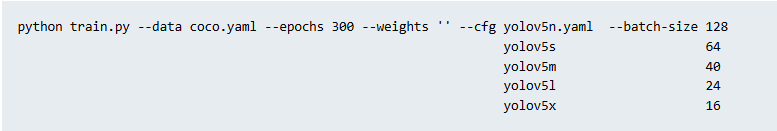
\includegraphics[width=0.8\textwidth]{picture/2.png}
    \caption{YOLOv5目标检测模型的训练命令}
\end{figure}
\subsubsection{测试自己制作的数据集}
从网上找寻了30张宝可梦的图片,然后通过labelImg工具\footnote{LabelImg 是一个开源的图像标注工具,用于创建图像数据集时标记图像中的对象边界框}标注这些图片中比较常见的宝可梦,如皮卡丘、杰尼龟等,然后将这些图片和标注文件放入到一个文件夹中。最后通过YOLOv5模型进行训练,得到了一个可以识别这些宝可梦的模型,因为数据集比较小,所以模型的识别率不是很高。
\\
\indent 训练结果示例:
\begin{figure}[H]
    \centering
    
\includegraphics[width=0.8\textwidth]{picture/3.png}
    \caption{YOLOv5目标检测模型的训练结果}
\end{figure}
\subsubsection{实现原理}
YOLOv5首先会在输入端中将输入图片进行预处理,图像大小调整为模型所需的大小,进行归一化操作,及将像素值缩放到0到1之间。\\
\indent 然后将图片输入到backbone网络\footnote{backbone网络是一个特征提取网络,用于提取图片的特征}中,backbone网络会将图片的特征提取出来,然后将这些特征输入到neck网络\footnote{neck网络是一个特征融合网络,用于将不同层次的特征进行融合}中,neck网络会将不同层次的特征进行融合,然后将这些特征输入到head网络\footnote{head网络是一个预测网络,用于预测图片中的物体}中,head网络会将图片中的物体进行预测,得到物体的类别和边界框。
\\
\indent 下图为YOLOv5的网络结构:
\footnote{CPL:由卷积Conv+批量归一化BN+激活函数Leaky Relu组成,用于在特征提取的过程中增加网络的信息传递能力。CPL通过在不同阶段的特征图之间进行部分连接,使得网络可以更充分地利用低级和高级特征,从而提高模型的性能。}
\footnote{CSP1:由CBL模块、Res uint模块以及卷积层Concat组成。CSP1是CPL的一种变体,它在CPL的基础上引入了跨阶段的残差连接,以进一步增强网络的信息传递能力。CSP1可以有效地减少网络中的计算量,提高模型的效率。}
\footnote{CSP2:不再使用Res unit,由卷积层CBL模块Concat组成。CSP2引入了路径重排的技术,以重新排列网络中的路径,使得前向和后向传播之间的信息流更加平滑和高效。这种路径重排有助于减少网络中的计算量,提高模型的速度和效率。CSP2同样也进行了路径融合(Path Fusion),即在不同路径之间进行信息融合,以使网络可以更充分地利用低级和高级特征。这种路径融合有助于提高模型对目标的检测和识别能力。CSP1也具有类似的路径融合机制。}
\footnote{SPP是一种用于空间金字塔池化的技术,它能够在不同尺度下提取图像的局部特征。SPP在YOLOv5中用于提取特征图的空间信息,从而使得模型可以更好地检测不同尺度和大小的目标。}
\footnote{Focus:对图像进行切片后再Concat}
\footnote{上采样:利用元素复制扩充的方法使得特征图尺寸扩大,例如线性插值。}
\footnote{Concat:张量拼接,会扩充两个张量的维度,实现多尺度特征融合。}
\begin{figure}[H]
    \centering
    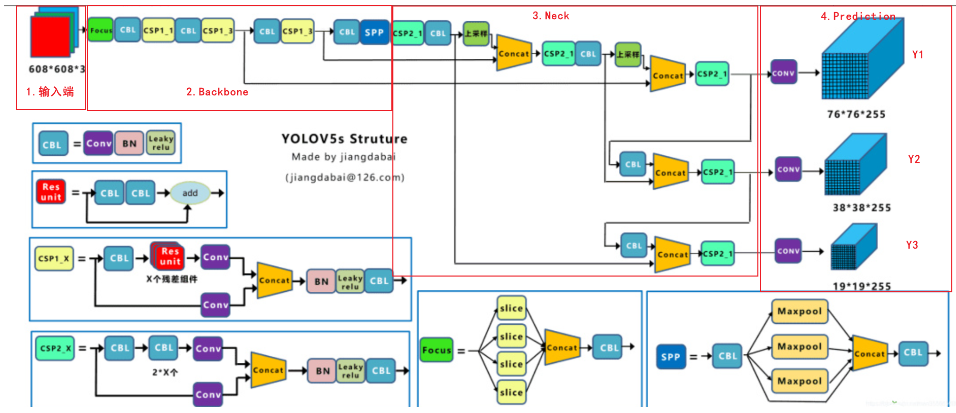
\includegraphics[width=0.8\textwidth]{picture/4.png}
    \caption{YOLOv5的网络结构}
\end{figure}
\makespace
\subsection{NeRF}
\subsubsection{模型简介}
NeRF(Neural Radiance Fields)是一种用于三维重建的深度学习模型,它可以从二维图像中重建出高质量的三维场景。NeRF的核心思想是利用神经网络来建模场景中每个空间点的辐射亮度和密度,从而实现对场景的准确重建。
\subsubsection{模型环境配置}
\noindent 于CUDA 10.2 基础下:
\begin{itemize}
    \item Python = 3.7.1
    \item cudatoolkit = 10.0.130
    \item tensorflow = 1.14.0
    \item numpy = 1.21.5
    \item imageio = 2.193
    \item configargparse = 1.4
\end{itemize}
模型从\underline{https://github.com/bmild/nerf.git}克隆下来,然后在本地进行配置。

\subsubsection{模型训练}
\indent 模型训练是在\underline{run\_nerf.py}文件中进行的,需要同时输入配置文件的的相对路径,配置文件中包含了实验名称(expname),基础目录(basedir),数据集路径(datadir),数据集类型(dataset\_type)采样参数、使用视角方向信息等模型训练和数据配置信息。

\subsubsection{训练结果}
先在730显卡的电脑上配置环境并尝试训练,但因预计训练结束时间要20左右,后改为在3080显卡的电脑上
重新配置环境。在重新配置环境时遇到一些版本冲突的问题,因为3080显卡的电脑上的CUDA版本是12.3,
不能与原配置的tensorflow版本1.14.0兼容,所以需要重新配置环境。最后在3080显卡的电脑上重新配置
环境并训练,但最后的预计训练结束时间人在一天左右,所以在github上找到了另外一个模型
NeRF Pytorch(详情见\hyperlink{section 2.3}{2.3 NeRF Pytorch})。
\makespace
\subsubsection{实现原理}
简单一点理解可以把NeRF看作是先用深度全连接神经网络(deep fully-connected neural network)\footnote{通常被称为多层感知机(
multilayer perceptron)或MLP,没有卷积层(convolutional layers),由全连接层(fully connected layer)和激活函数(activation 
function)组成}去学习并训练一个静态3D场景,实现复杂场景的任意新视角合成(渲染)。NeRF的核心思想是将静态场景表示为5D函数,即每个空间点
x$(x,y,z)$和方向d$(\theta\footnote{极角(Polar Angle),通常的取值范围是0到π之间,通常表示从参考方向(通常是参考坐标系的正方向)
到目标向量(或目标位置)的角度,简单一点可以理解为与z轴的夹角}, \phi\footnote{方位角(Azimuthal Angle),通常的取值范围是0到2π之间,
通常表示目标向量在参考平面上投影与参考方向的夹角,简单一点可以理解为在xy平面上与x轴的夹角})$都对应一个颜色(RGB)和密度$(\sigma)$。
NeRF的输入是一条被5D函数代表的射线,输出是射线上每个点的颜色和密度。其中方向d$(\theta,\phi)$,在进入模型前将先会被展开成三维笛卡尔坐
标(3D Cartesian)系下的单位向量\(\vec{u}\)。这种单位向量可以用来表示一个方向,它有着确定的$x,y,z$三个分量,记为$(ux, uy, uz)$。由于是
单位向量,所以这三个分量要满足(公式2.1):
\begin{equation}
    \begin{aligned}
        u_x^2 + u_y^2 + u_z^2 = 1
        \captionsetup{labelformat=default}
    \end{aligned}
\end{equation}
$(ux, uy, uz)$具体的计算公式如下(公式2-2):
\begin{equation}
    \begin{aligned}
        u_x &= \sin(\theta)\cos(\phi)\\
        u_y &= \sin(\theta)\sin(\phi)\\
        u_z &= \cos(\theta)
    \end{aligned}
\end{equation}
\indent
在进入模型前, 通常还会先将$(x,y,z)$和$(ux, uy, uz)$通过位置编码(positional encoding)\footnote{位置编码是一种将空间位置信息映射到
更高维的空间中的技术,它可以帮助模型更好地理解空间位置信息,从而提高模型的性能。}映射到更高维的周期性函数空间\footnote{周期性函数空间是
指由周期函数构成的函数空间。一个周期性函数$f(x)$是指满足$f(x+T) = f(x)$的函数,其中$T$是一个常数,称为周期。}中,以增加模型的表达能力。
转换公式示例如下(公式2-3):
\begin{equation}
    \begin{aligned}
        r(x) &= (\sin(2^0\pi x), \cos(2^0\pi x), \sin(2^1\pi x), \cos(2^1\pi x), \cdots, \sin(2^{L-1}\pi x), \cos(2^{L-1}\pi x))
    \end{aligned}
\end{equation}
\indent
及将一个一维向量$x$映射到一个$2L$维的向量,在论文中作者对空间点$x(x,y,z)$转换成了60维的向量,即$L=10$,$3 \times 2L(L=10) = 60$,
同时将方向d从3维$(ux, uy, uz)$转换成了24维的向量,即$L=4$,$3 \times 2L(L=4) = 24$。
(详情见\hyperlink{图2-5}{图2-5})。下图为论文实验时使用位置编码和不使用位置编码的对比图(图2-4):
\begin{figure}[H]
    \centering
    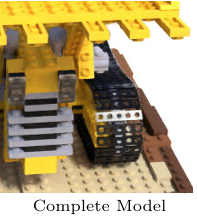
\includegraphics[width=0.4\textwidth]{picture/6.png}
    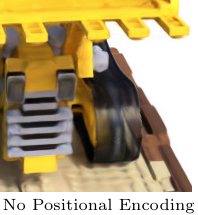
\includegraphics[width=0.4\textwidth]{picture/7.png}
    \caption{使用位置编码和不使用位置编码的对比图}
\end{figure}
\indent
从上图中可以看出在使用了位置编码后,模型在细节的表达中会更好,尤其是在凹凸不平的地方,而不使用位置编码的模型在这些地方会变得模糊。\\
\\
\indent
在实际使用位置编码时除了上述公式中的$2L$维向量外,有时还会加上一个维度为1的向量和表示其本身的向量进行拼接成为$2L+2$维的向量(论文的实验中
并未使用$2L+2$维的向量,这里仅仅只是补充说明),这两个向量的加入可以帮助模型更好的学习低频平滑部分,同时提高模型的灵活性。加入后的新向量
如下(公式2-4):
\begin{equation}
    \begin{aligned}
        r(x) &= (\sin(2^0\pi x), \cos(2^0\pi x), \sin(2^1\pi x), \cos(2^1\pi x), \cdots, \sin(2^{L-1}\pi x), \cos(2^{L-1}\pi x), x, 1)
    \end{aligned}
\end{equation}
\indent
空间点$x(x,y,z)$通过位置编码升维过后的高维向量会先进入深度全连接神经网络(MLP)中,在经过多层的全连接层和激活函数(Activation Function)
\footnote{激活函数的作用是在神经网络中引入非线性因素,使得整个网络由线性变换的组合升级为非线性变换的组合,从而能够拟合更加复杂的映射函数。
没有激活函数,即使是深层网络,最终的输出也只能是输入的线性组合,表达能力是有限的。}
后,最后输出密度($\sigma$)和 一个维度和之前全连接层维度相同的中间特征向量,中间特征会和三维方向向量d通过位置编码升维过后的高维向量一起
输入到额外的全连接层中去预测颜色(RGB)。示例如下图(图2-5):
\hypertarget{图2-5}{}
\begin{figure}[H]
    \centering
    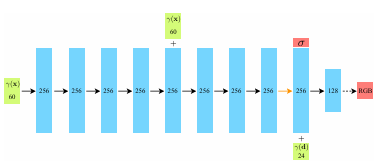
\includegraphics[width=0.8\textwidth]{picture/5.png}
    \caption{NeRF中的MLP结构示例}
\end{figure}
在论文中(如上图)作者使用了8层的全连接层,每层的隐藏单元数为256,激活函数为ReLU(Rectified Linear Unit),空间点$x(x,y,z)$在进入这个8
层的全连接层后输出了密度($\sigma$)和一个维度为256的中间特征向量。这个中间特征向量和和方向d一起进入一层额外的全连接层中去预测颜色(RGB、
),这个额外的全连接层包含了激活函数ReLU和128个隐藏单元。其中ReLU激活函数的公式为(公式2-5):
\begin{equation}
    \begin{aligned}
        f(x) = \max(0,x)
    \end{aligned}
\end{equation}
表面上来看ReLU只是简单的将小于0的值截为0,但实际上它引入了一个分段线性的非线性函数:
\begin{enumerate}
    \item 当输入大于0时,ReLU(x)=0,输出是一个常量
    \item 当输入小于0时,ReLU(x)=x,输出与输入是线性关系
\end{enumerate}
这两个分段线性区域的接合点$(x=0)$引入了一个折线的不连续点,使得整个映射函数不再是单纯的线性方程,而具有了非线性的性质。如下图(图2-6):
\begin{figure}[H]
    \centering
    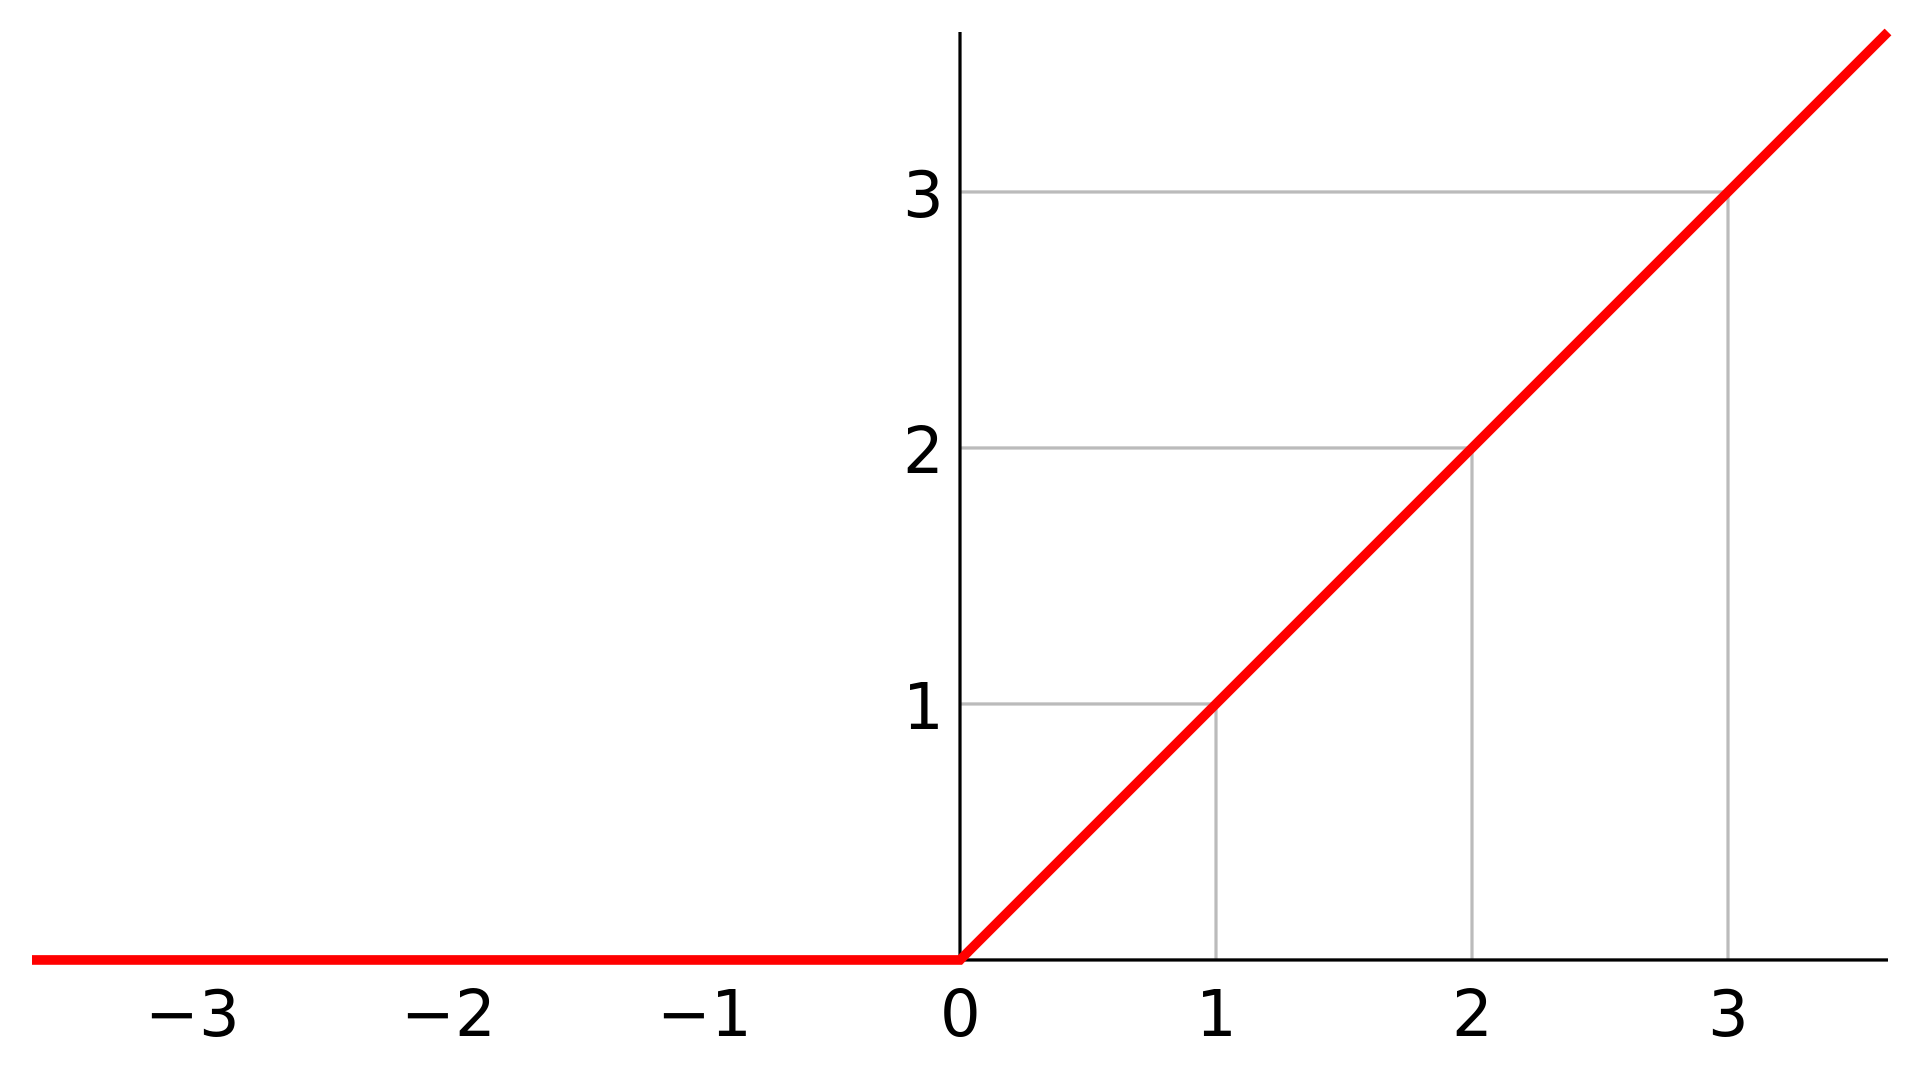
\includegraphics[width=0.8\textwidth]{picture/8.png}
    \caption{ReLU激活函数示例}
\end{figure}
\makespace
\hypertarget{section 2.3}{}
\subsection{NeRF Pytorch}
\makespace
\section*{致谢}
\begin{center}
    { \blackti \fontsize{16.0600pt}{1.25}致 \, 谢}
\end{center}
\addcontentsline{toc}{section}{致\texorpdfstring{ \, }{} 谢}
\myspace{1}
致谢内容。

\makespace
\section*{文献}
\begin{center}
    { \blackti \fontsize{16.0600pt}{1.25}文 \, 献}
\end{center}
\addcontentsline{toc}{section}{文\texorpdfstring{ \, }{} 献}
\myspace{1}
\noindent
Mildenhall, B., Srinivasan, P. P., Tancik, M., Barron, J. T., Ramamoorthi, R., \& Ng, R. (2020). NeRF: 
Representing Scenes as Neural Radiance Fields for View Synthesis. In European Conference on Computer Vision 
(ECCV).\\
\end{document}

